\section{Anhang}

\subsection{Wei�lichtpunkt}
\label{subsec:weisslicht}
Fit (Abbildung \ref{fig:weisslichtpunkt_eichung_1}) und Parameter (Tabelle \ref{tab:weisslichtpunkt_eichung_1}) f�r die ersten Wei�lichtpunkt.

\begin{figure}[H]
\centering
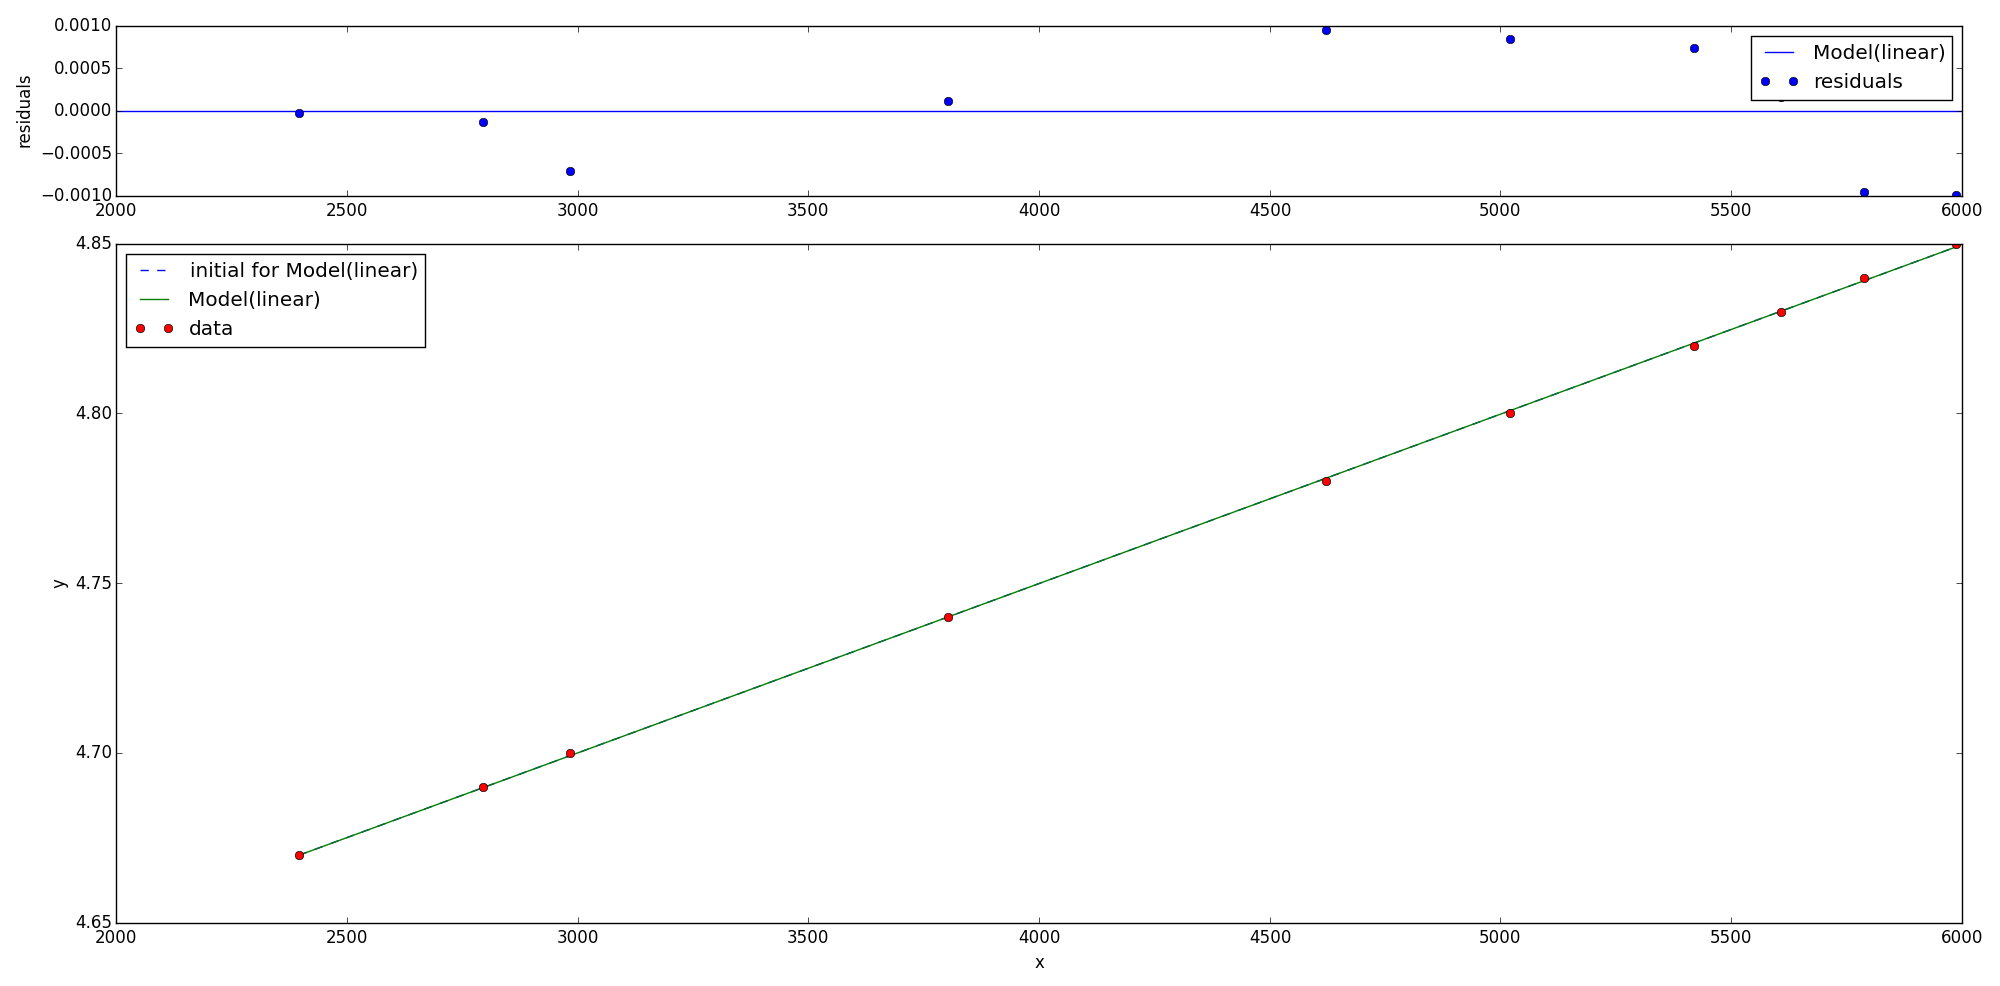
\includegraphics[scale = 0.33]{eichung_weisslicht_4,75.png}
\caption{Erster bestimmter Wei�punkt bei 4,7545(8) $\mu$m}
\label{fig:weisslichtpunkt_eichung_1}
\end{figure}

\begin{table}[H]
\centering
\caption{Parameter des Fits f�r den ersten Wei�lichtpunkt}
\label{tab:weisslichtpunkt_eichung_1}
\begin{tabular}{|c|c|}
\hline Parameter & Wert \\ 
\hline A & 4.98(2)e-05 \\ 
\hline B & 4.5505(9) \\ 
\hline 
\end{tabular} 
\end{table}

Fit (Abbildung \ref{fig:weisslichtpunkt_eichung_2}) und Parameter (Tabelle \ref{tab:weisslichtpunkt_eichung_2}) f�r die zweiten Wei�lichtpunkt.

\begin{figure}[H]
\centering
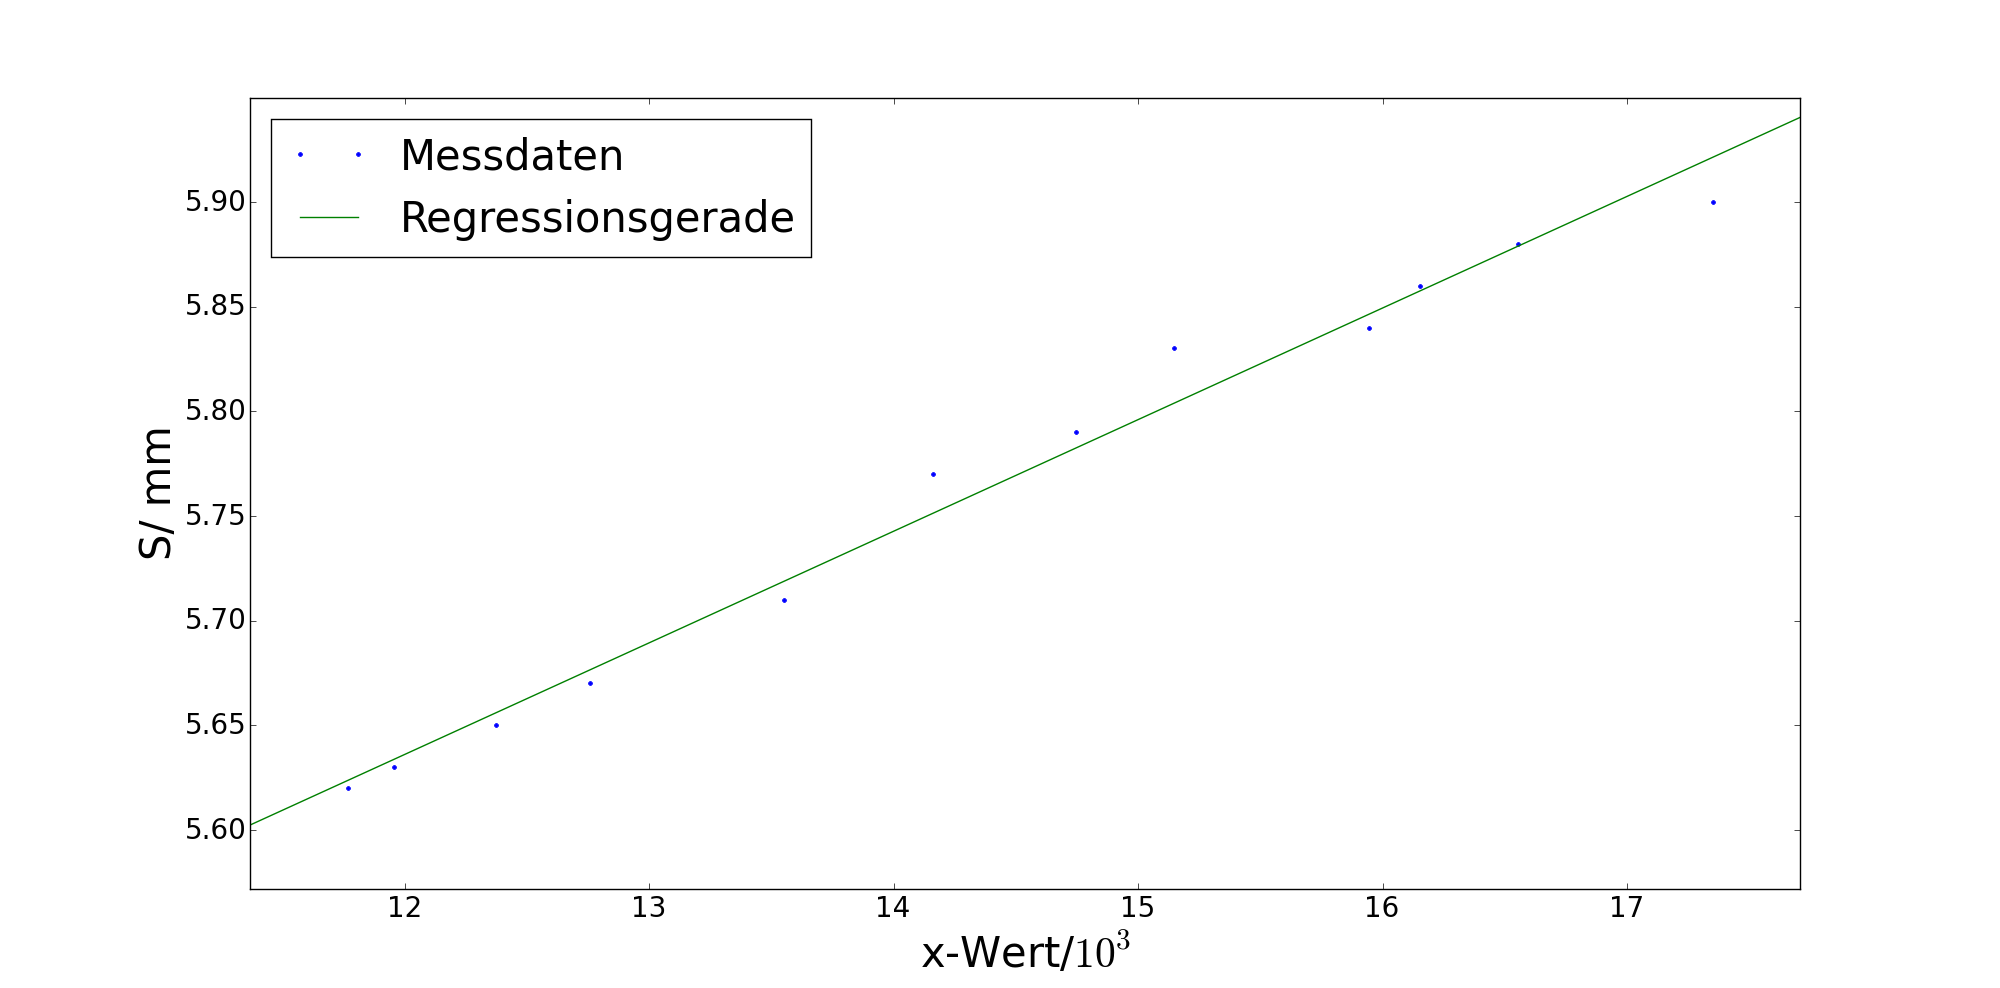
\includegraphics[scale = 0.33]{eichung_weisslicht_5,77.png}
\caption{Erster bestimmter Wei�punkt bei 5,77(3) $\mu$m}
\label{fig:weisslichtpunkt_eichung_2}
\end{figure}

\begin{table}[H]
\centering
\caption{Parameter des Fits f�r den zweiten Wei�lichtpunkt}
\label{tab:weisslichtpunkt_eichung_2}
\begin{tabular}{|c|c|}
\hline Parameter & Wert \\ 
\hline A & 4.98(2)e-05 \\ 
\hline B & 4.5505(9) \\ 
\hline 
\end{tabular} 
\end{table}
\subsection{Schwebung}
\label{Schwebung}
\begin{figure}[H]
\centering
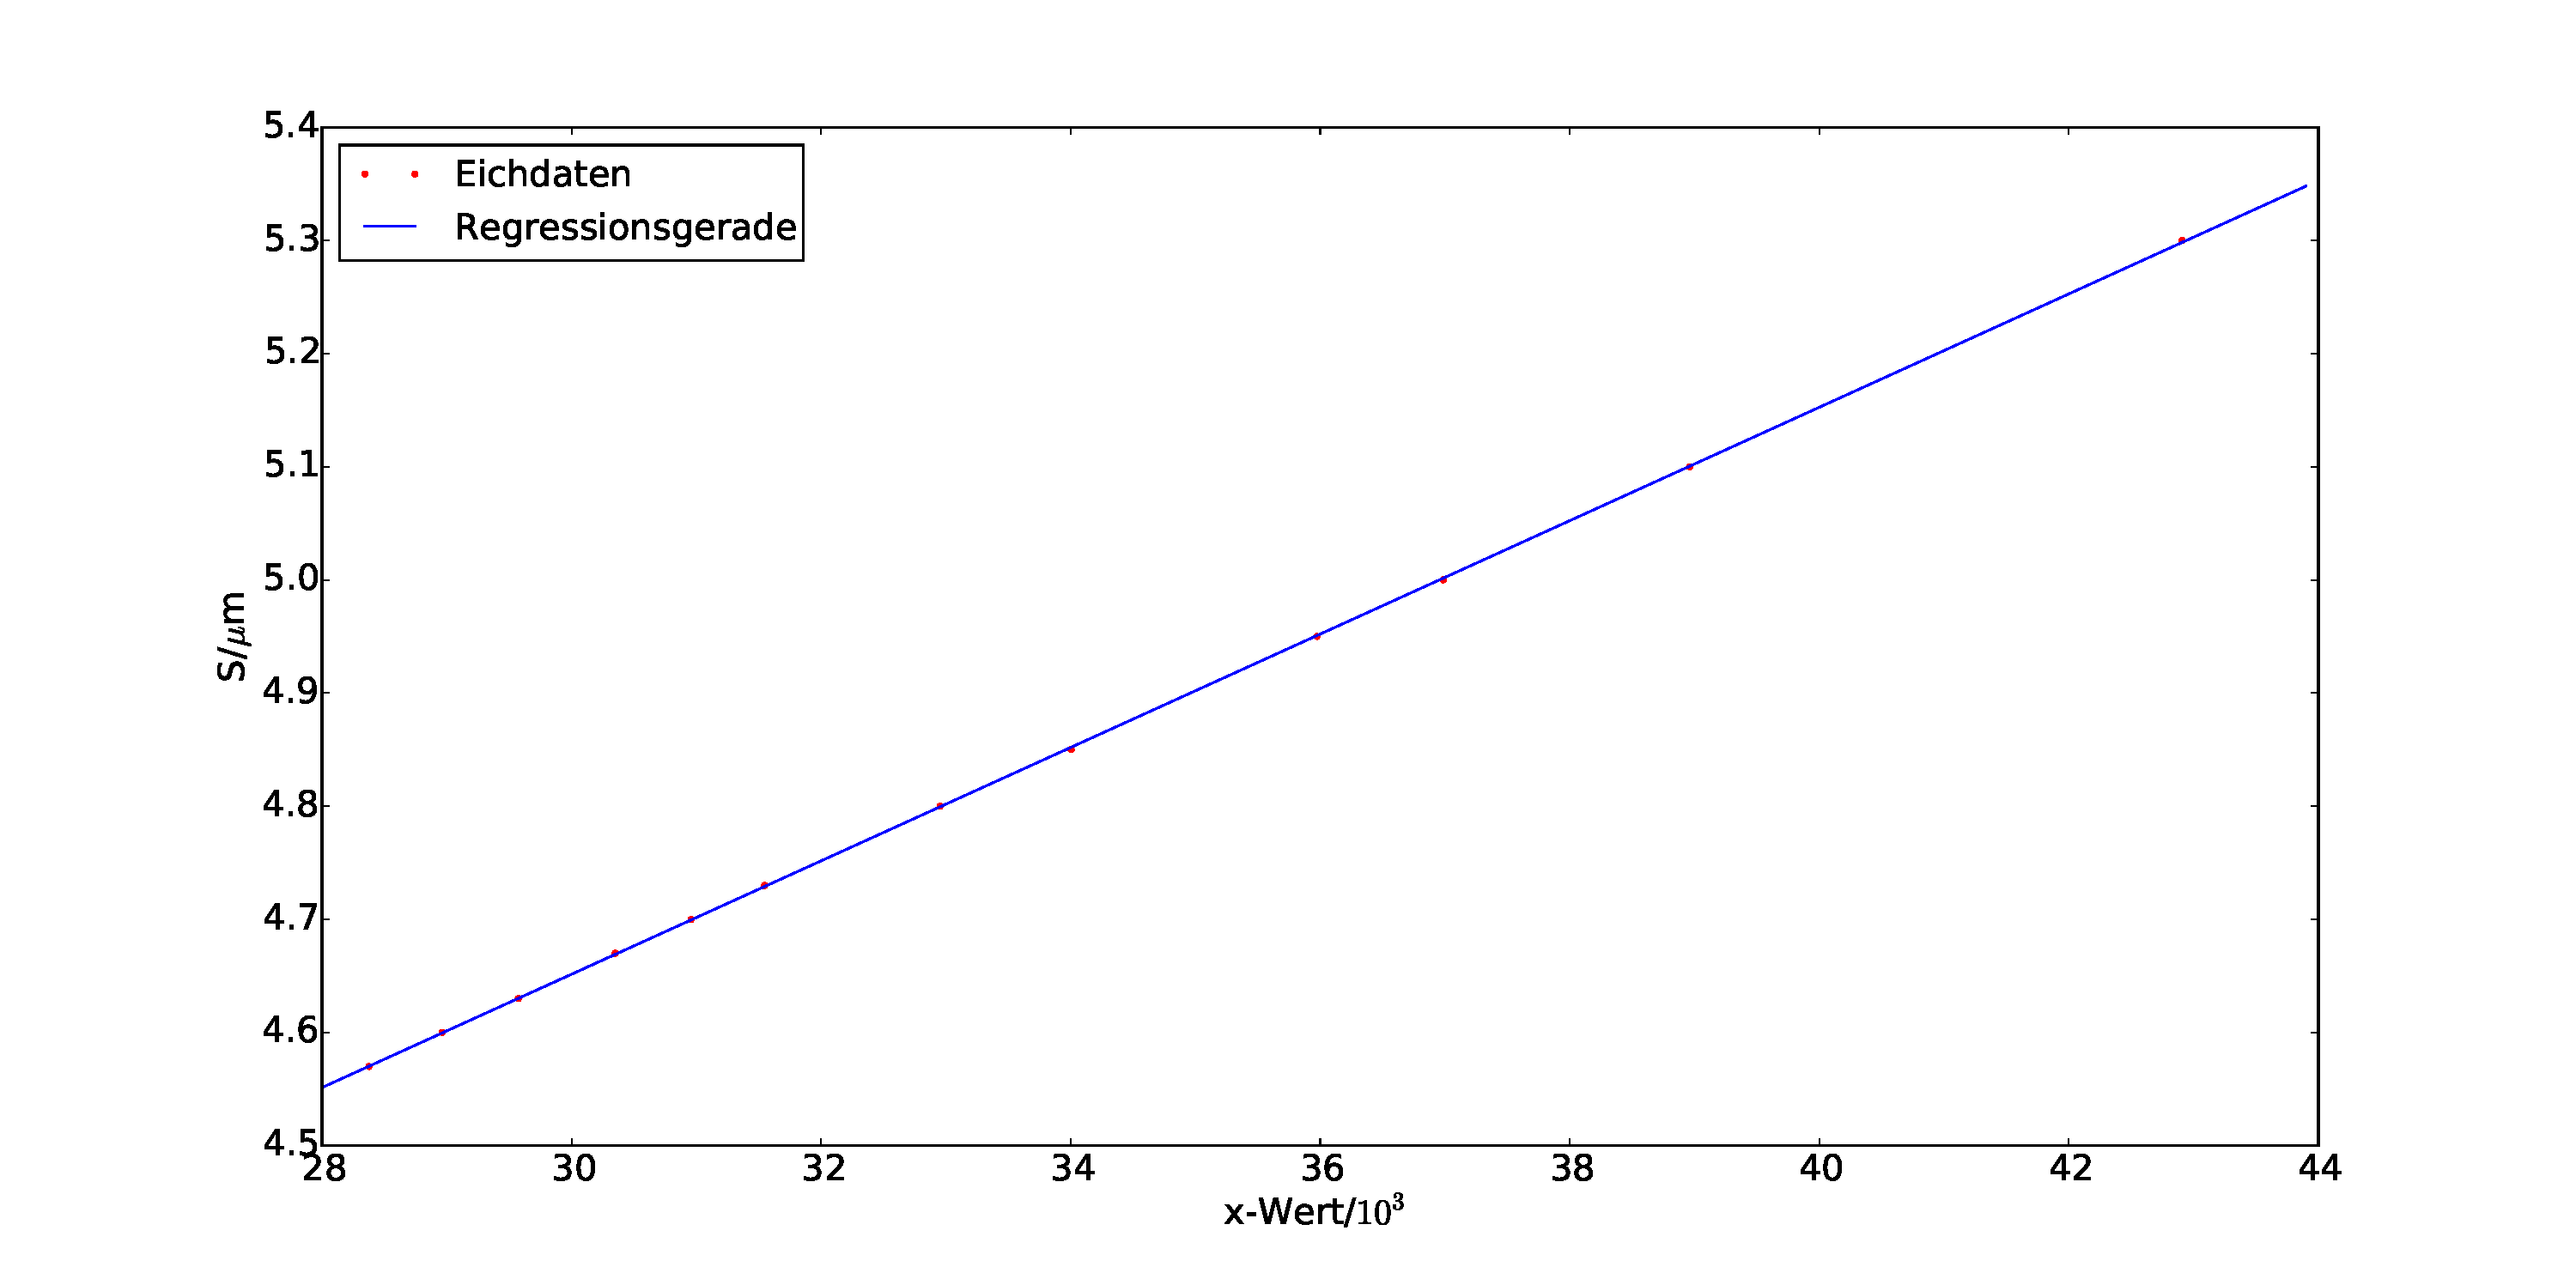
\includegraphics[scale = 0.33]{Eichdaten_Schwebung}
\caption{Eichung f�r die Schwebung mit einer Fitfunktion $S(x)/\mu m= 5,010(8)\cdot10^{-5}\cdot x + 3.1485(26)$. F�r die Berechnung des Fits wurde der Ursprung in den Schwerpunkt der Daten gelegt, um f�r den Fit unkorrelierte Fitparameter zu erhalten.}
\label{fig:Schwebung_Eichung}
\end{figure}